\documentclass[8pt,a4paper]{extarticle}
\usepackage[margin=.8cm,bottom=10mm]{geometry}
\usepackage[utf8]{inputenc}
\usepackage[IL2]{fontenc}
\usepackage[czech]{babel}
\usepackage{microtype}
\usepackage{amssymb}
\usepackage{amsthm}
\usepackage{amsmath}
\usepackage{xcolor}
\usepackage{graphicx}
\usepackage{wasysym}
\usepackage{multicol}
\usepackage[inline]{enumitem}

\multicolsep=\smallskipamount

\newcommand{\R}{\mathbb{R}}
\newcommand{\N}{\mathbb{N}}
\newcommand{\Z}{\mathbb{Z}}

\newcommand{\hint}[1]{{\color{gray}\footnotesize\noindent(Nápověda: #1)}}

\DeclareMathOperator{\tg}{tg}
\DeclareMathOperator{\cotg}{cotg}

\setlist[enumerate]{label={(\alph*)},topsep=\smallskipamount,itemsep=\smallskipamount,parsep=0pt,itemjoin={\quad}}
\setlist[itemize]{topsep=\smallskipamount,noitemsep}

\def\tisk{%
\newbox\shipouthackbox
\pdfpagewidth=2\pdfpagewidth
\let\oldshipout=\shipout
\def\shipout{\afterassignment\zdvojtmp \setbox\shipouthackbox=}%
\def\zdvojtmp{\aftergroup\zdvoj}%
\def\zdvoj{%
    \oldshipout\vbox{\hbox{%
        \copy\shipouthackbox
        \hskip\dimexpr .5\pdfpagewidth-\wd\shipouthackbox\relax
        \box\shipouthackbox
    }}%
}}%

\let\results\newpage
\let\endresults\relax

\def\resultssame{%
    \long\def\results##1\endresults{%
        \vfill
        \noindent\rotatebox{180}{\vbox{##1}}%
    }%
}


\newtheorem*{poz}{Pozorování}

\theoremstyle{definition}
\newtheorem{uloha}{\atr Úloha}
\newtheorem{suloha}[uloha]{\llap{$\star$ }Úloha}
\newtheorem*{bonus}{Bonus}
\newtheorem*{defn}{Definice}

\pagestyle{empty}

\DeclareMathOperator{\arctg}{arctg}

\let\=\doteq
\let\ee\expandafter

\def\vysld{}
\let\printvysl\relax
\let\printalphvysl\relax

\makeatletter
\long\def\vyslplain#1{\ee\ee\ee\gdef\ee\ee\ee\vysld\ee\ee\ee{\ee\vysld\ee\printvysl\ee{\the\c@uloha}{#1}}}
\let\vysl\vyslplain

\def\locvysl#1{\ee\gdef\ee\locvysld\ee{\locvysld\item #1}}
\let\lv\locvysl

\newenvironment{ulohav}[1][]{\begin{uloha}[#1]\gdef\locvysld{\begin{enumerate*}}}{\ee\vyslplain\ee{\locvysld\end{enumerate*}}\end{uloha}}
\def\stitem{\@noitemargtrue\@item[$\star$ \@itemlabel]}

\makeatother

\def\atr{}
\def\basic{\def\atr{\llap{\mdseries$\sun$\,}\gdef\atr{}}}
\def\sinterest{\def\atr{\llap{$(\star)$\,}\gdef\atr{}}}
\def\interest{\def\atr{\llap{$\star$\,}\gdef\atr{}}}
\def\iinterest{\def\atr{\llap{$\star\star$\,}\gdef\atr{}}}
\let\mb\mathbf

\def\ms{\,\mathrm{m}\cdot\mathrm{s}^{-1}}

\mathcode`\,="013B

\def\st{^\circ}

\begin{document}

% \tisk
% \resultssame

\section*{18. Sinová a kosinová věta}

\begin{itemize}[itemsep=\smallskipamount]
\item sinová věta: $\dfrac{a}{\sin \alpha} = \dfrac{b}{\sin \beta} = \dfrac{c}{\sin \gamma} = 2r$;%
\quad
kosinová věta: $c^2 = a^2 + b^2 - 2ab\cos \gamma$
\item užitečná pravidla: $\alpha+\beta+\gamma=180\st$;\quad proti delší straně je větší úhel (a naopak); \quad trojúhelníková nerovnost
\end{itemize}

\begin{multicols}{2}

\begin{ulohav}[kosinová věta -- délky]
Určete všechny možné délky třetí strany ve (standardně značeném) trojúhelníku $ABC$, víte-li následující; uveďte výsledky s přesností na čtyři desetinná místa, pokud není uvedeno jinak.
\begin{enumerate}
    \item $a = 5$, $b = 6$, $\gamma = 29\st$\lv{$c \= 2,9194$}
    \item $c = 3,73$, $a = 1,28$, $\beta = 32\st5'17''$\lv{$b \=2,7315$}
    \item $b = \sqrt2$, $c = \sqrt{18}$, $\alpha = 60\st$ (spočtěte přesně!)\lv{$a = \sqrt{14}$}
    \item $a = 13$, $b = 7$, $\alpha = 70\st$\lv{$c \= 13,6072$}
    \item $b = 11$, $c = 5$, $\gamma = 25\st$\lv{$a_1 \= 8,1286$, $a_2 \= 11,8102$ (dvě řešení)}
    \item $b = 13$, $c = 2$, $\gamma = 40\st$\lv{nemá řešení -- takový $\triangle$ neexistuje}
\end{enumerate}
\end{ulohav}


\begin{ulohav}[kosinová věta -- úhly]
Určete velikosti všech vnitřních úhlů s~přesností na úhlové vteřiny v trojúhelníku $ABC$, víte-li
\begin{enumerate}
    \item $a = 2$, $b = 3$, $c = 4$\lv{$\alpha \= 28\st57'18''$, $\beta \= 46\st34'3''$, $\gamma \= 104\st 28' 39''$}
    \item $a = 3$, $b = 8$, $c = 4$\lv{takový $\triangle$ neexistuje (není splněna $\triangle$ nerovnost)}
\end{enumerate}
\end{ulohav}


\begin{ulohav}[sinová věta -- délky]
Určete délku strany $a$ v~trojúhelníku $ABC$, víte-li
\begin{enumerate}
    \item $\alpha = 53\st$, $b = 3$, $\beta = 19\st$\lv{$\= 7,3591$}
    \item $c = 43,137$, $\gamma = 46\st13'13''$, $\alpha = 111\st52'18''$\lv{$\=55,4456$}
    \item $\alpha = 45\st$, $\beta = 60\st$, $b = 3$ (spočtěte přesně!)\lv{$\sqrt6$}
    \item $\alpha = 112\st$, $\gamma = 76\st$, $c = 6$\lv{takový $\triangle$ neexistuje (příliš velký součet úhlů)}
\end{enumerate}
\end{ulohav}


\begin{ulohav}[sinová věta -- úhly]
Určete všechny možné velikosti úhlu $\alpha$ v~trojúhelníku $ABC$, víte-li
\begin{multicols}{2}
\begin{enumerate}
    \item $a = 5$, $b = 4$, $\beta = 47\st$\lv{cca $66\st5'29''$ nebo $113\st54'31''$}
    \item $a = 5$, $b = 6$, $\beta = 47\st$\lv{cca $37\st33'2''$ (druhý možný výsledek je větší než $\beta$)}
    \item $a = 2$, $b = 7$, $\beta = 47\st$\lv{cca $12\st3'41''$ (druhý možný výsledek je větší než $\beta$)}
    \item $a = 7$, $b = 2$, $\beta = 47\st$\lv{takový $\triangle$ neexistuje (vyjde $\sin \alpha > 1$)}
    \item $a = 5$, $b = 2$, $\beta = 160\st$\lv{takový $\triangle$ neexistuje (oba výsledky menší než $\beta$)}
    \item $a = 4$, $b = 3$, $\beta = 10\st$\lv{cca $13\st23'14''$ nebo $166\st36'46''$}
\end{enumerate}
\end{multicols}
\end{ulohav}


\begin{uloha}
Kružnice opsaná trojúhelníku má poloměr $5$. Jak velký vnitřní úhel může být naproti straně o délce $7$? \vysl{cca $44\st25'37''$ nebo $135\st34'23''$}
\end{uloha}


\begin{ulohav}[\uv{řešte trojúhelníky}]
Dopočtěte velikosti všech stran a vnitřních úhlů ve standardně značeném trojúhelníku $ABC$, máte-li zadané následující údaje; nalezněte \emph{všechna} řešení. Délky určujte s přesností na 4 desetinná místa a velikosti úhlů s přesností na úhlové vteřiny.
\begin{multicols}{2}
\begin{enumerate}
    \item $a = 5$, $\beta = 55^\circ$, $\gamma = 65^\circ$
        \lv{$\alpha = 60^\circ$, $b\=4,7294$, $c \= 5,2326$}
    \item $a = 4$, $c = 5$, $\beta = 40^\circ$
        \lv{$b\=3,2184$, $\alpha\=53\st1'26''$, $\gamma\=86\st58'34''$}
    \item $b = 11$, $c = 6$, $\alpha = 13\st$
        \lv{$a \= 5,3276$, $\beta \= 152\st19'28''$, $\gamma \= 14\st40'32''$}
    \item $a = 3$, $c = 4$, $\alpha = 30^\circ$
        \lv{(I)~$\gamma_1 \= 41\st48'37''$, $\beta_1 \= 108\st11'23''$, $b_1 \= 5,7002$ nebo (II)~$\gamma_2 \= 138\st11'23''$, $\beta_2 \= 11\st48'37''$, $b_2 \= 1,2208$}
    \item $b = 21$, $c = 25$, $\beta = 81^\circ$
        \lv{$\triangle$ neexistuje}
    \item $a = 7$, $b = 4$, $\alpha = 100^\circ$
        \lv{$\beta \= 34\st14'46''$, $\gamma \= 45\st45'14''$, $c \= 5,0918$}
    \item $a = 7$, $v_a = 5,5$, $\gamma = 115\st$
        \lv{$b \= 6,0686$, $c \= 11,0333$, $\alpha \= 35\st5'59''$, $\beta \= 29\st54'1''$}
    \item $c = 10$, $t_a = 17$, $\beta=132^\circ$
        \lv{$a \= 17,1967$, $b \= 25,0173$, $\alpha \= 30\st43'10''$, $\gamma \= 17\st16'50''$}
\end{enumerate}
\end{multicols}
\end{ulohav}


\begin{multicols}{2}
\begin{uloha}
Síly $\mb F_1$ a $\mb F_2$ mají společné působiště, velikosti 8\,N a 5\,N a svírají úhel $\varphi = 37\st$. Jakou velikost má výslednice $\mb F$ těchto sil a jaký úhel svírá se silou $\mb F_1$?
\vysl{velikost $\= 12,3649$\,N, úhel $\= 14\st5'5''$}
\end{uloha}
\hbox{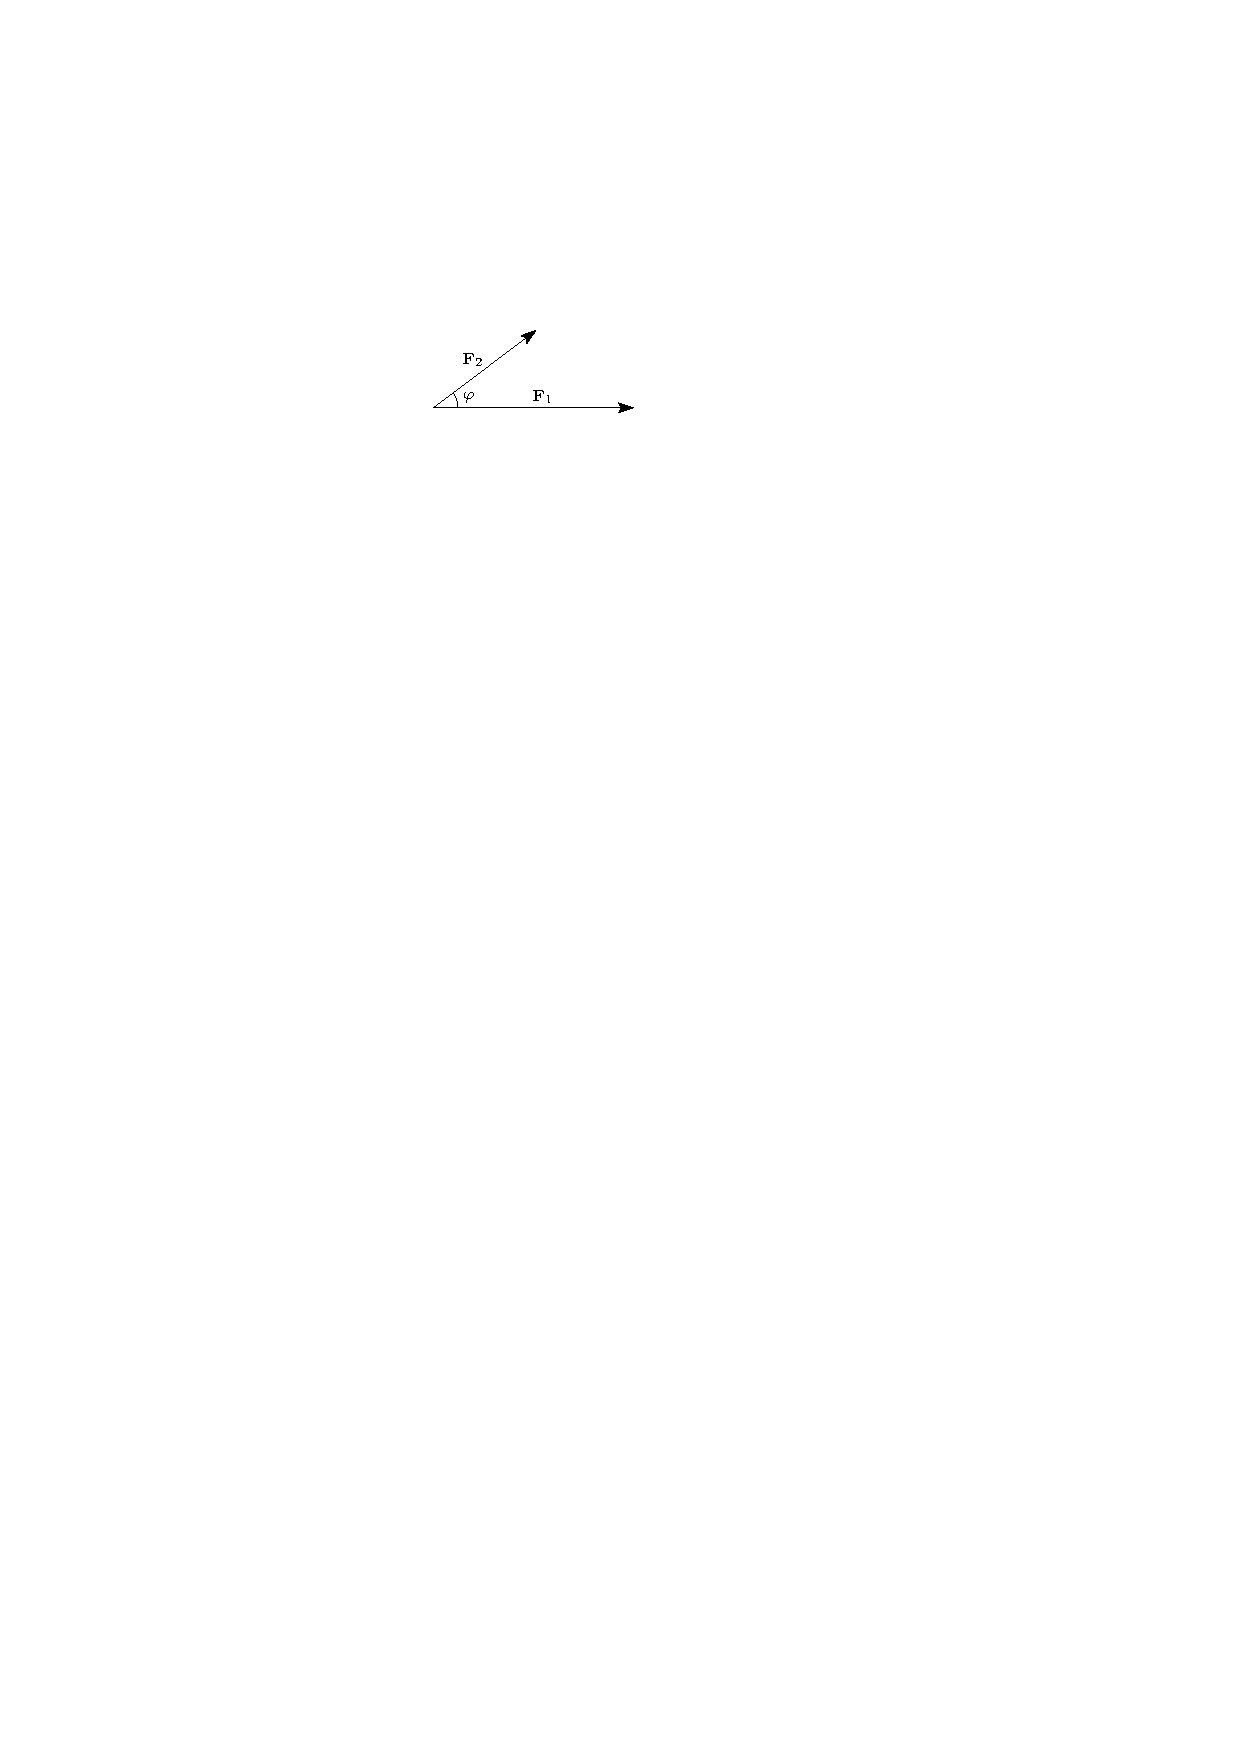
\includegraphics{sily.pdf}}
\end{multicols}


\interest
\begin{uloha}
Určete obecně, jakou velikost bude mít výslednice dvou sil o velikostech $F_1$, $F_2$, které svírají (konvexní) úhel $\varphi$.
\vysl{$\sqrt{F_1^2 + F_2^2 + 2 F_1 F_2 \cos\varphi}$}
\end{uloha}


\begin{uloha} % pracák Didaktisu
Koumák Karel chce zjistit výšku topolu, který se nachází v~sousedovic zahradě za plotem.
Vrchol topolu vidí z~určitého místa ve výškovém úhlu $22^\circ$. Když se (po vodorovné rovině) přiblíží směrem k~topolu o $40$\,m, vidí jeho vrchol ve výškovém úhlu $45^\circ 12'$. Jak vysoký je topol?
\vysl{cca 26,9898\,m}
\end{uloha}


\begin{uloha} % pracák Didaktisu
Určete výměru pozemku na obrázku a délky obou jeho úhlopříček. \hint{Na výpočet obsahu se může hodit Heronův vzorec.} \vysl{obsah cca $7084,2233\,\mathrm{m}^2$, úhlopříčky mají délky cca $137,3414$\,m a $109,3134$\,m}
\[ 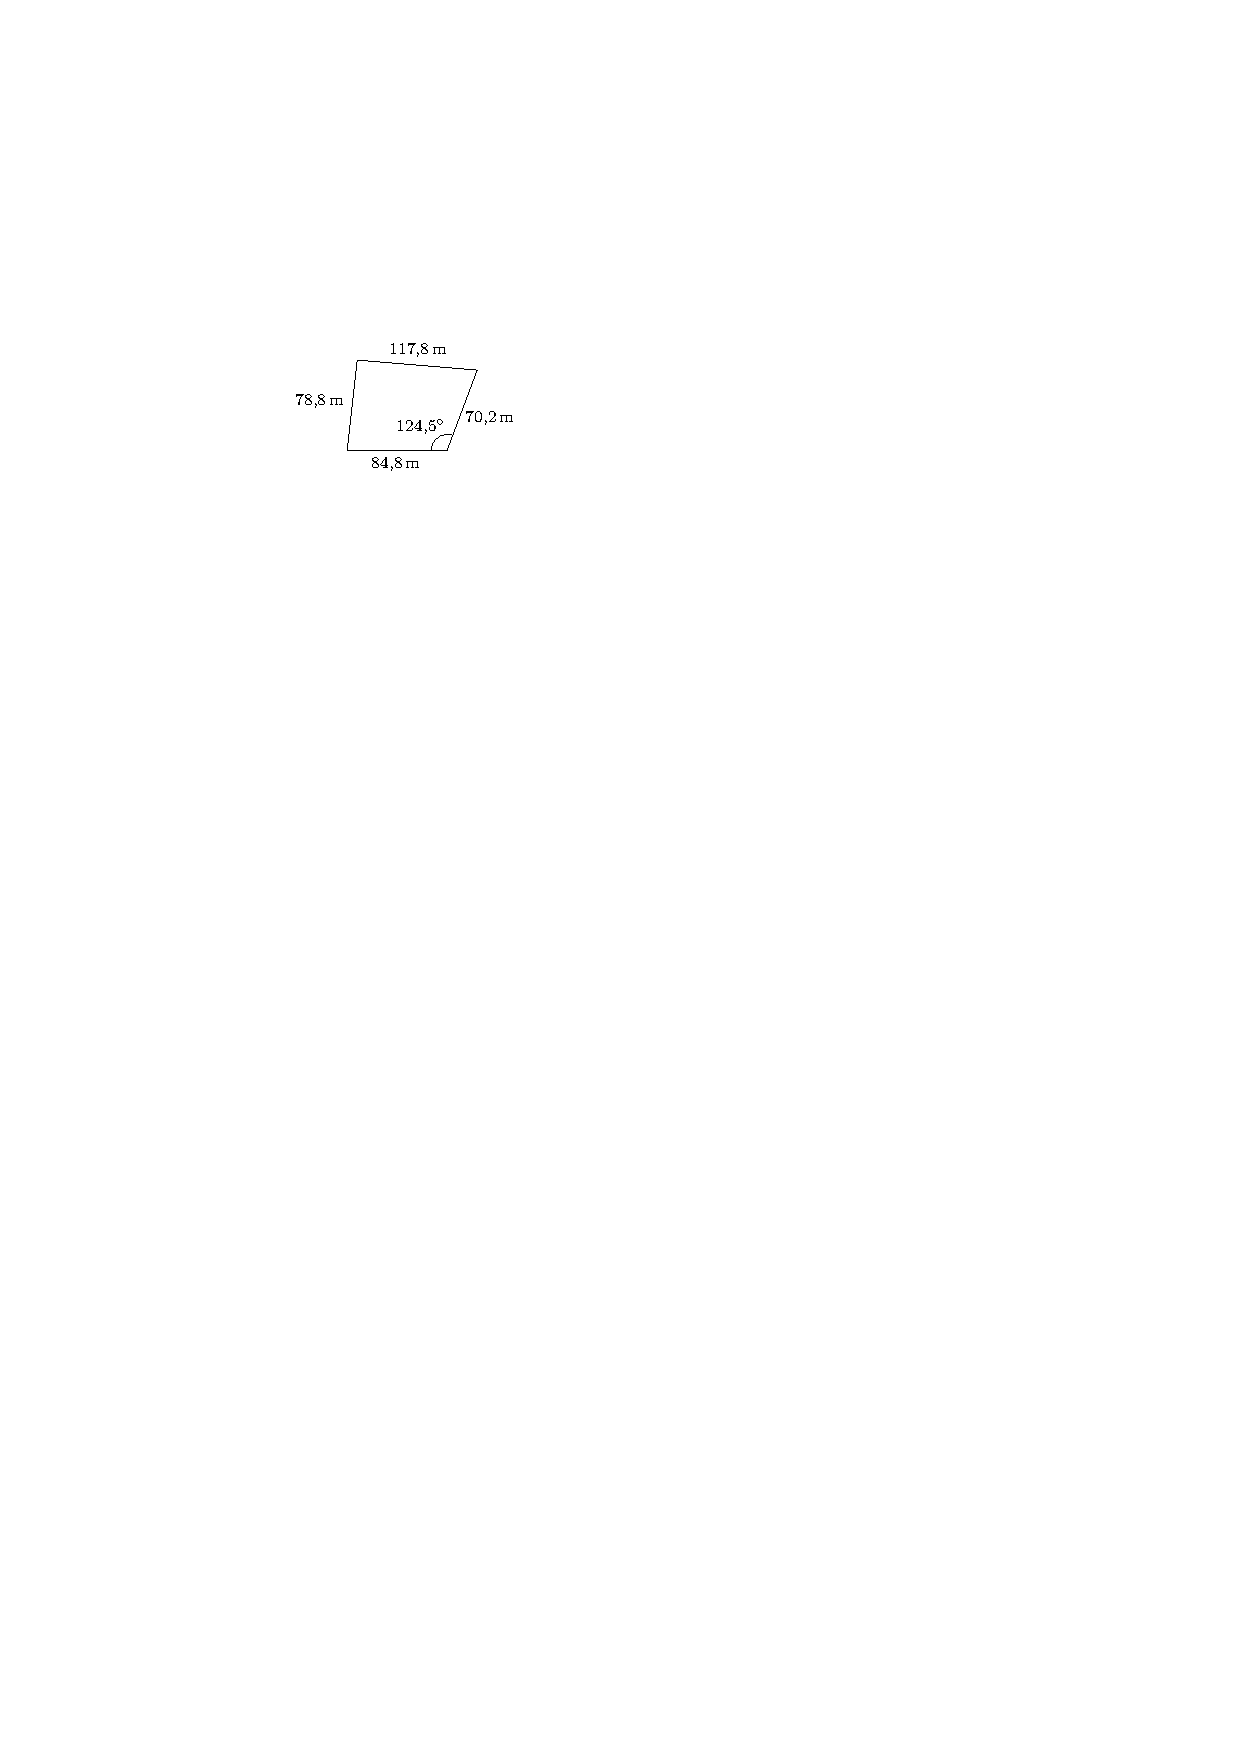
\includegraphics{pozemek.pdf} \]
\end{uloha}


\begin{ulohav}
Vítr způsobuje, že letadla typicky neletí \uv{rovnou za nosem}, ale jsou při přímém letu snášena na nějakou stranu. Aby tedy letadlo letělo tam, kam chceme, musí vliv větru kompenzovat určitou odchylkou od zamýšleného směru. Výsledná rychlost letadla vůči zemi (včetně směru) je pak vektorovým součtem rychlosti větru vůči zemi a teoretické rychlosti letadla za bezvětří.

Jestliže vítr fouká rychlostí $17\ms$ pod azimutem $31^\circ$, pilot chce letět ve směru $130^\circ$ (tj. toto má být výsledný reálný směr) a rychlost letadla za bezvětří je $150\ms$, určete:
\begin{enumerate}
    \item jak moc a na jakou stranu má být letadlo natočeno od svého reálného směru letu,
        \lv{musí se natočit doprava cca o $6\st25'37''$ od směru, jakým chce letět}
    \item jak velká (v $\!\ms$) bude skutečná rychlost letadla vůči zemi.
        \lv{cca $146,3979\ms$}
\end{enumerate}
Poznámka: Azimut se měří od severu po směru hodinových ručiček.
\end{ulohav}


\begin{ulohav}
Jestliže ve standardně značeném trojúhelníku $ABC$ platí $a = 3$, $b=10$, určete všechny velikosti úhlu $\alpha$, pro které
\begin{enumerate}[noitemsep]
    \item budou existovat právě dva takové trojúhelníky, \lv{$\alpha \in (0^\circ; \arcsin\frac{3}{10})$}
    \item bude existovat právě jeden takový trojúhelník, \lv{$\alpha  = \arcsin\frac{3}{10}$}
    \item nebude existovat žádný takový trojúhelník. \lv{$\alpha \in (\arcsin\frac{3}{10}; 180^\circ)$}
\end{enumerate}
\hint{Spíš si to zkuste nakreslit, až pak počítejte.}
\end{ulohav}


\interest
\begin{uloha}
Určete obvod trojúhelníku $ABC$, pokud platí $a+b=30$, $\alpha = 35^\circ$, $\beta = 66^\circ$. \vysl{$a \= 11,57$, $b \= 18,43$, $c \= 19,8$, $o \= 49,8$}
\end{uloha}


\interest
\begin{uloha}
Pomocí sinové a kosinové věty určete hodnoty $\sin 75\st$ a $\cos 75\st$ (neboli $\sin \frac{5\pi}{12}$ a $\cos \frac{5\pi}{12}$).
Návod: Uvažte trojúhelník s vnitřními úhly $\alpha = 45\st$, $\beta = 60\st$, $\gamma = 75\st$. Zafixujte velikost jedné strany (např. $a=1$), dopočtěte sinovou větou $b$, kosinovou větou $c$ a nakonec sinovou větou $\sin \gamma$ a kosinovou větou $\cos \gamma$.\vysl{$\sin 75\st = \frac{\sqrt6 + \sqrt2}{4}$, $\cos 75\st = \frac{\sqrt6 - \sqrt2}{4}$}
\end{uloha}


\interest
\begin{uloha}[důkaz kosinové věty]
Dokažte kosinovou větu -- např. pomocí tohoto obrázku:
\[ 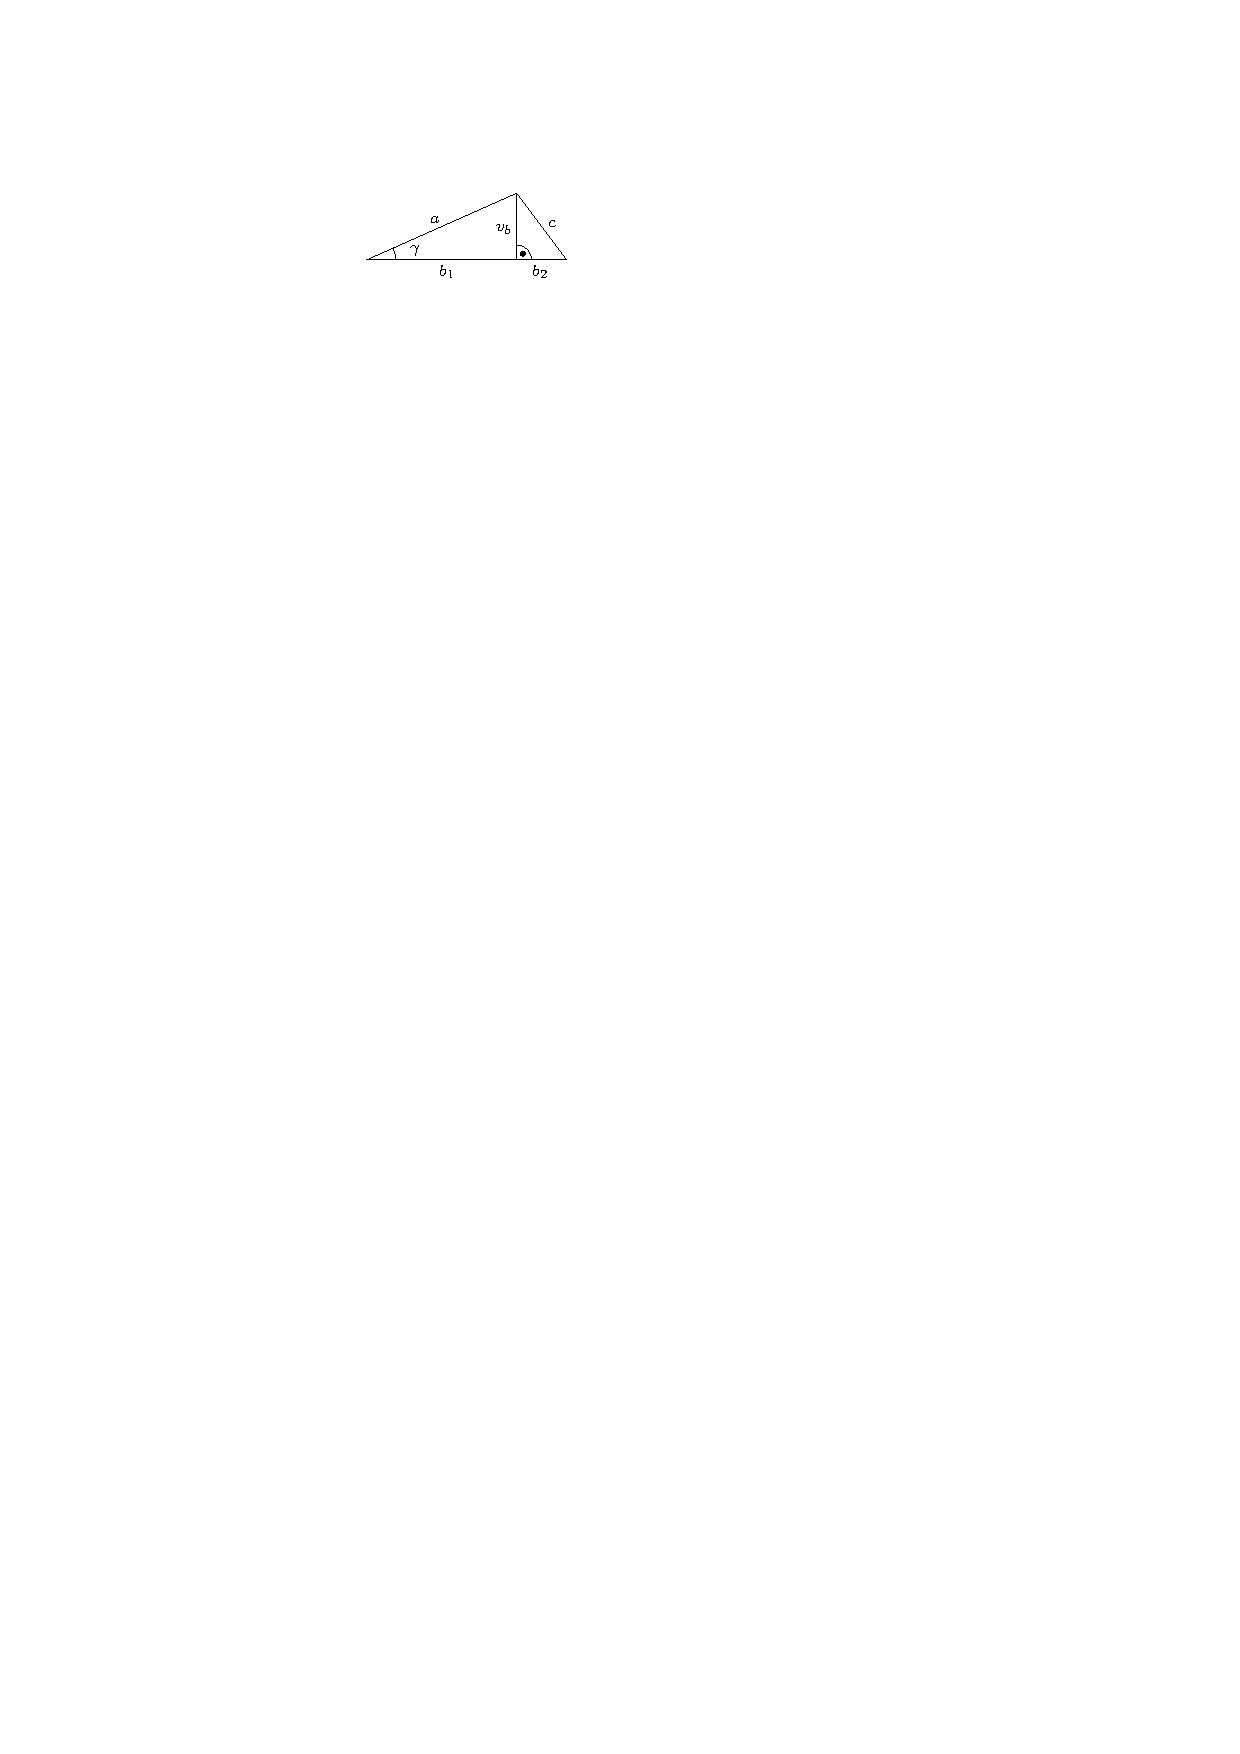
\includegraphics{dukaz_cos.pdf} \]
Co by se změnilo, kdyby se výška $v_b$ nacházela vně trojúhelníka?
\end{uloha}


\interest
\begin{uloha}[důkaz sinové věty]
Dokažte sinovou větu -- např. s využitím faktu, že pokud v trojúhelníku $ABC$ \uv{hýbeme} bodem $A$ po kružnici opsané, tak se velikost úhlu $\sphericalangle BAC$ buď nemění, nebo se změní na doplněk do $180\st$ (důsledek věty o středovém a obvodovém úhlu) + Thaletovy věty.
\end{uloha}

\end{multicols}


\setlist[enumerate]{label={{\bfseries(\alph*)}},itemjoin={\quad}}

\results
\parindent=0pt
\parskip=\smallskipamount
\rightskip=0pt plus1fil\relax
\def\printvysl#1#2{\textbf{#1.} #2\par}
\begin{multicols}{2}
\vysld
\end{multicols}
\endresults


\end{document}